\newpage
\section*{Exercise 3 (Comments made by Qahir)}
For code see appendix. 10000 samples were run. 

On figure \ref{fig:ex31} the samples along with the true pdf for the exponential, normal and Pareto with support $\geq 1$ can be seen. And on figure \ref{fig:ex32} the results for Pareto distributions with support $\geq 0$ can be seen. For the exponential and standard normal we have a good correspondence. For the Pareto it is generally seen that the lower values of $k$ are more difficult to sample from both in the case with support $\geq 1$ and support $\geq 0$. By use of the theoretical formula one can calculate the variances and expectations for the pareto with support $\geq 1$. Here has that the expectation should be $1.952$ and variance should be $37.188$ for $k=2.05$, for $k=4.0$ these should be $1.333$ and $0.2222$ respectively. From the samples for $k=2.05$ the mean is $1.94$ and variance $4.74$. For $k=4$ these are $1.333$ and $0.222$. From this it can be seen that it is more difficult to make inference for lower values of $k$ compared to higher. This is because the Pareto distribution has undefined variance for $k \leq 2$. The closer the parameter $k$ gets to this value the more difficult it will be to perform inference. 


\begin{figure}[H]
        \centering
        \begin{subfigure}[H]{0.475\textwidth}
            \centering
            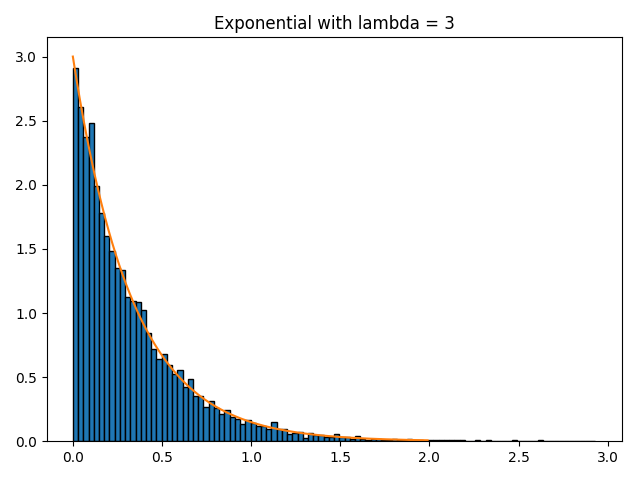
\includegraphics[width=\textwidth]{exp.png}
            \caption[Network2]%
            {{\small Exponential with $\lambda = 3$}}    
            \label{fig:mean and std of net14}
        \end{subfigure}
        \hfill
        \begin{subfigure}[H]{0.475\textwidth}  
            \centering 
            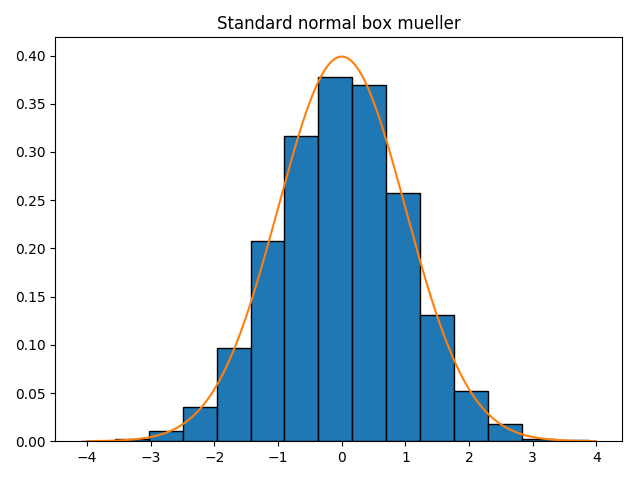
\includegraphics[width=\textwidth]{normal.png}
            \caption[]%
            {{\small Samples of standard normal using box-mueller}}    
            \label{fig:mean and std of net24}
        \end{subfigure}
        \vskip\baselineskip
        \begin{subfigure}[H]{0.475\textwidth}   
            \centering 
            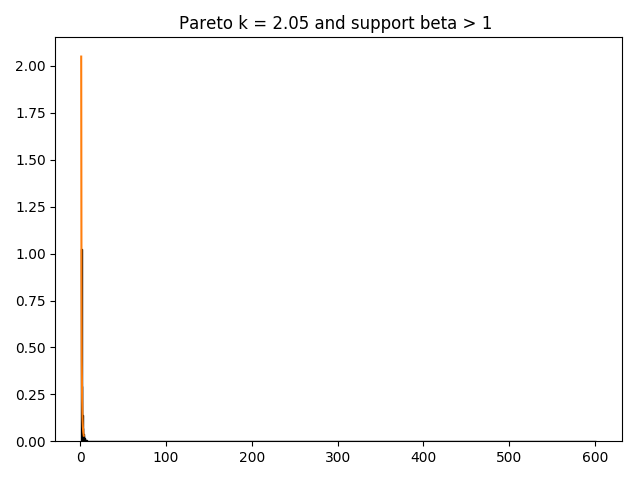
\includegraphics[width=\textwidth]{pars1.png}
            \caption[]%
            {{\small Pareto with support $ \geq 1$ and $k=2.05$}}    
            \label{fig:mean and std of net34}
        \end{subfigure}
        \quad
        \begin{subfigure}[H]{0.475\textwidth}   
            \centering 
            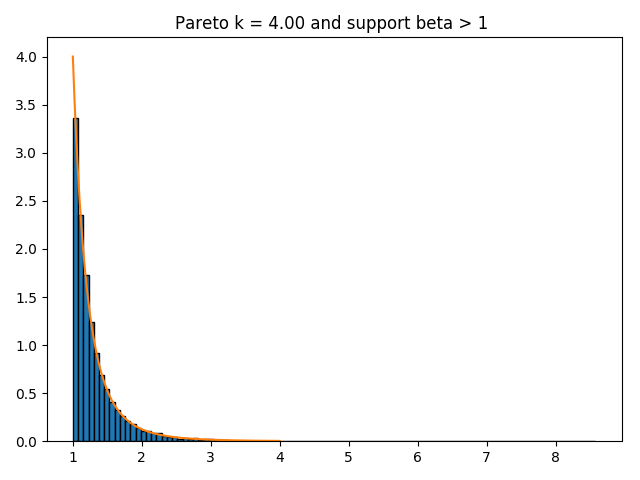
\includegraphics[width=\textwidth]{pars2.png}
            \caption[]%
            {{\small Pareto with support $ \geq 1$ and $k=4.0$}}    
            \label{fig:stuff}
        \end{subfigure}
        \caption[ The average and standard deviation of critical parameters ]
        {\small Histogram of different sampling methods (blue) - the orange line indicate the true pdf} 
        \label{fig:ex31}
    \end{figure}


\begin{figure}[H]
        \centering
        \begin{subfigure}[H]{0.475\textwidth}
            \centering
            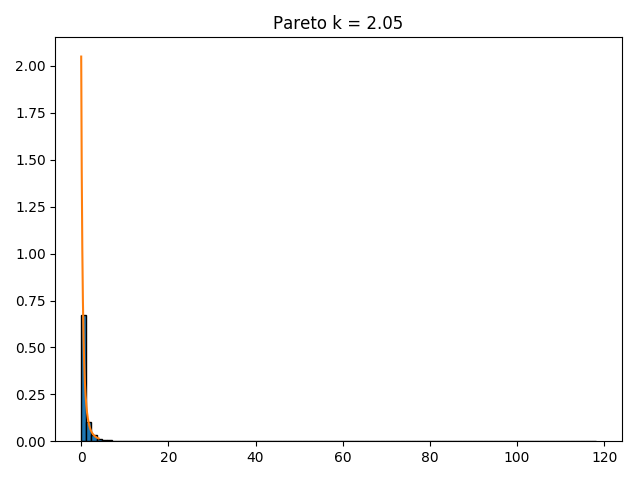
\includegraphics[width=\textwidth]{par1.png}
            \caption[Network2]%
            {{\small Pareto with support $\geq 0$ and $k=2.05$}}    
            \label{fig:mean and std of net14}
        \end{subfigure}
        \hfill
        \begin{subfigure}[H]{0.475\textwidth}  
            \centering 
            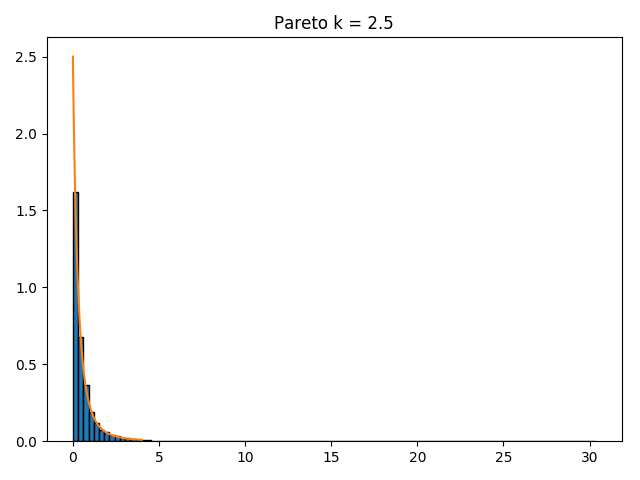
\includegraphics[width=\textwidth]{par2.png}
            \caption[]%
            {{\small Pareto with support $\geq 0$ and $k=2.50$}}    
            \label{fig:mean and std of net24}
        \end{subfigure}
        \vskip\baselineskip
        \begin{subfigure}[H]{0.475\textwidth}   
            \centering 
            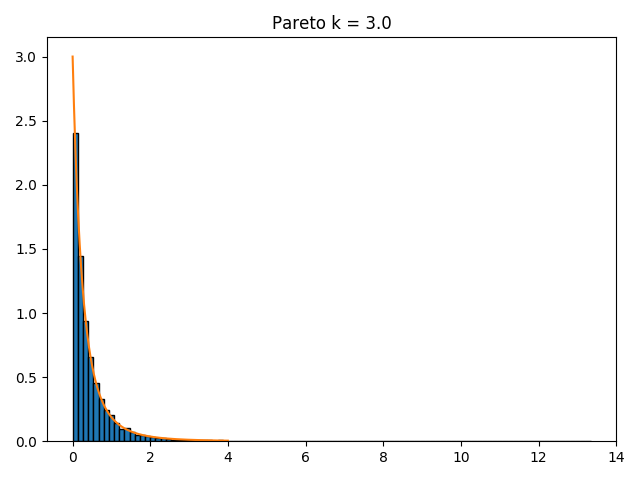
\includegraphics[width=\textwidth]{par3.png}
            \caption[]%
            {{\small Pareto with support $\geq 0$ and $k=3.00$}}    
            \label{fig:mean and std of net34}
        \end{subfigure}
        \quad
        \begin{subfigure}[H]{0.475\textwidth}   
            \centering 
            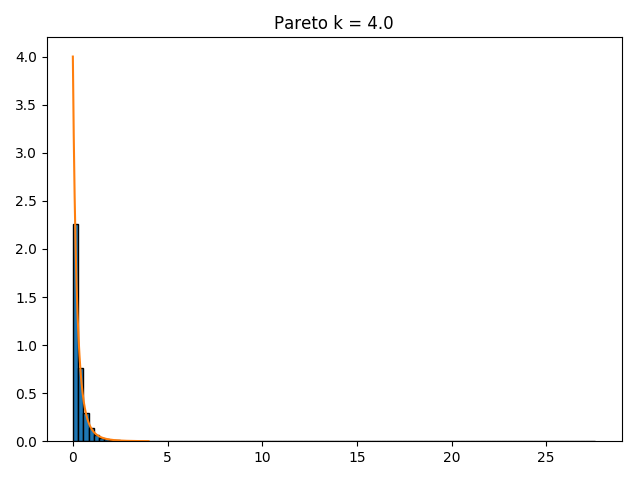
\includegraphics[width=\textwidth]{par4.png}
            \caption[]%
            {{\small Pareto with support $\geq 0$ and $k=4.0$}}    
            \label{fig:stuff}
        \end{subfigure}
        \caption[ The average and standard deviation of critical parameters ]
        {\small Histogram of different sampling methods (blue) - the orange line indicate the true pdf} 
        \label{fig:ex32}
    \end{figure}

A confidence interval for the mean and variance of a standard normal distribution was also made. This was done by using the code for the standard Box Mueller procedure. $100$ iterations were run with $10$ samples in each. The respective $95\%$-confidence intervals were estimated from the quantiles. Here it was found that for the mean the CI was $[-0.5891,0.6535]$ and for the variance $[0.285, 1.982]$. The true values are inside the confidence interval but the length of the interval is quite large. Performing less iterations and running with more samples in each iteration will probably decrease the width of the confidence interval. A KS-test testing the different distributions was also performed and can be seen on \ref{tab:ex3}. It is seen that all the p-values are all above the significance level $0.05$ and hence we cannot reject that all the samples come from their respective distributions. The test was done using stats.kstest in numpy. Here the function 'lomax' corresponds to our parametrization of the Pareto with support $\geq 0$ and 'pareto' corresponds to our parametrization with support $\geq 1$. For code used see appendix. 

\begin{table}[H]
    \centering
    \begin{tabular}{|c|c|} \hline
    Name & $p$-value  \\ \hline
    Normal Box Mueller & 0.622 \\ \hline
    Exponential & 0.96 \\ \hline
    Pareto ($k=2.05$ and support $\geq1$) & 0.130 \\ \hline
    Pareto ($k=4.0$ and support $\geq 1$) & 0.1245 \\ \hline
    Pareto $k=2.05$ & 0.72 \\ \hline
    Pareto $k=2.50$ & 0.93 \\ \hline
    Pareto $k=3.0$ & 0.40 \\ \hline
    Pareto $k=4.0$ & 0.257 \\ \hline
    \end{tabular}
    \caption{KS - test}
    \label{tab:ex3}
\end{table}